\chapter{Konwolucyjna sieć incepcja}
\label{chap:inception}

\section{Architektura sieci incepcja}

\subsection{Wstęp}
Siec Incepcja (\textit{ang. Inception Network}) została zaprezentowana w 2015 roku w publikacji \textit{ang. Going deeper with convolutions} \cite{inceptionpaper}. 
Nazwa sieci (wraz z tytułem publikacji) nawiązuje do popularnego w tamtym czasie internetowego mema z Leonardo DiCaprio. 
Incepcja wychodzi na przeciw problemom z treningiem bardzo głębokich sieci neuronowych. Jednym z nich jest rosnący margines błędu wraz rosnącą ilością warstw co przedstawia rysunek \ref{fig:deep-error}.

\begin{figure}[ht]
\centerline{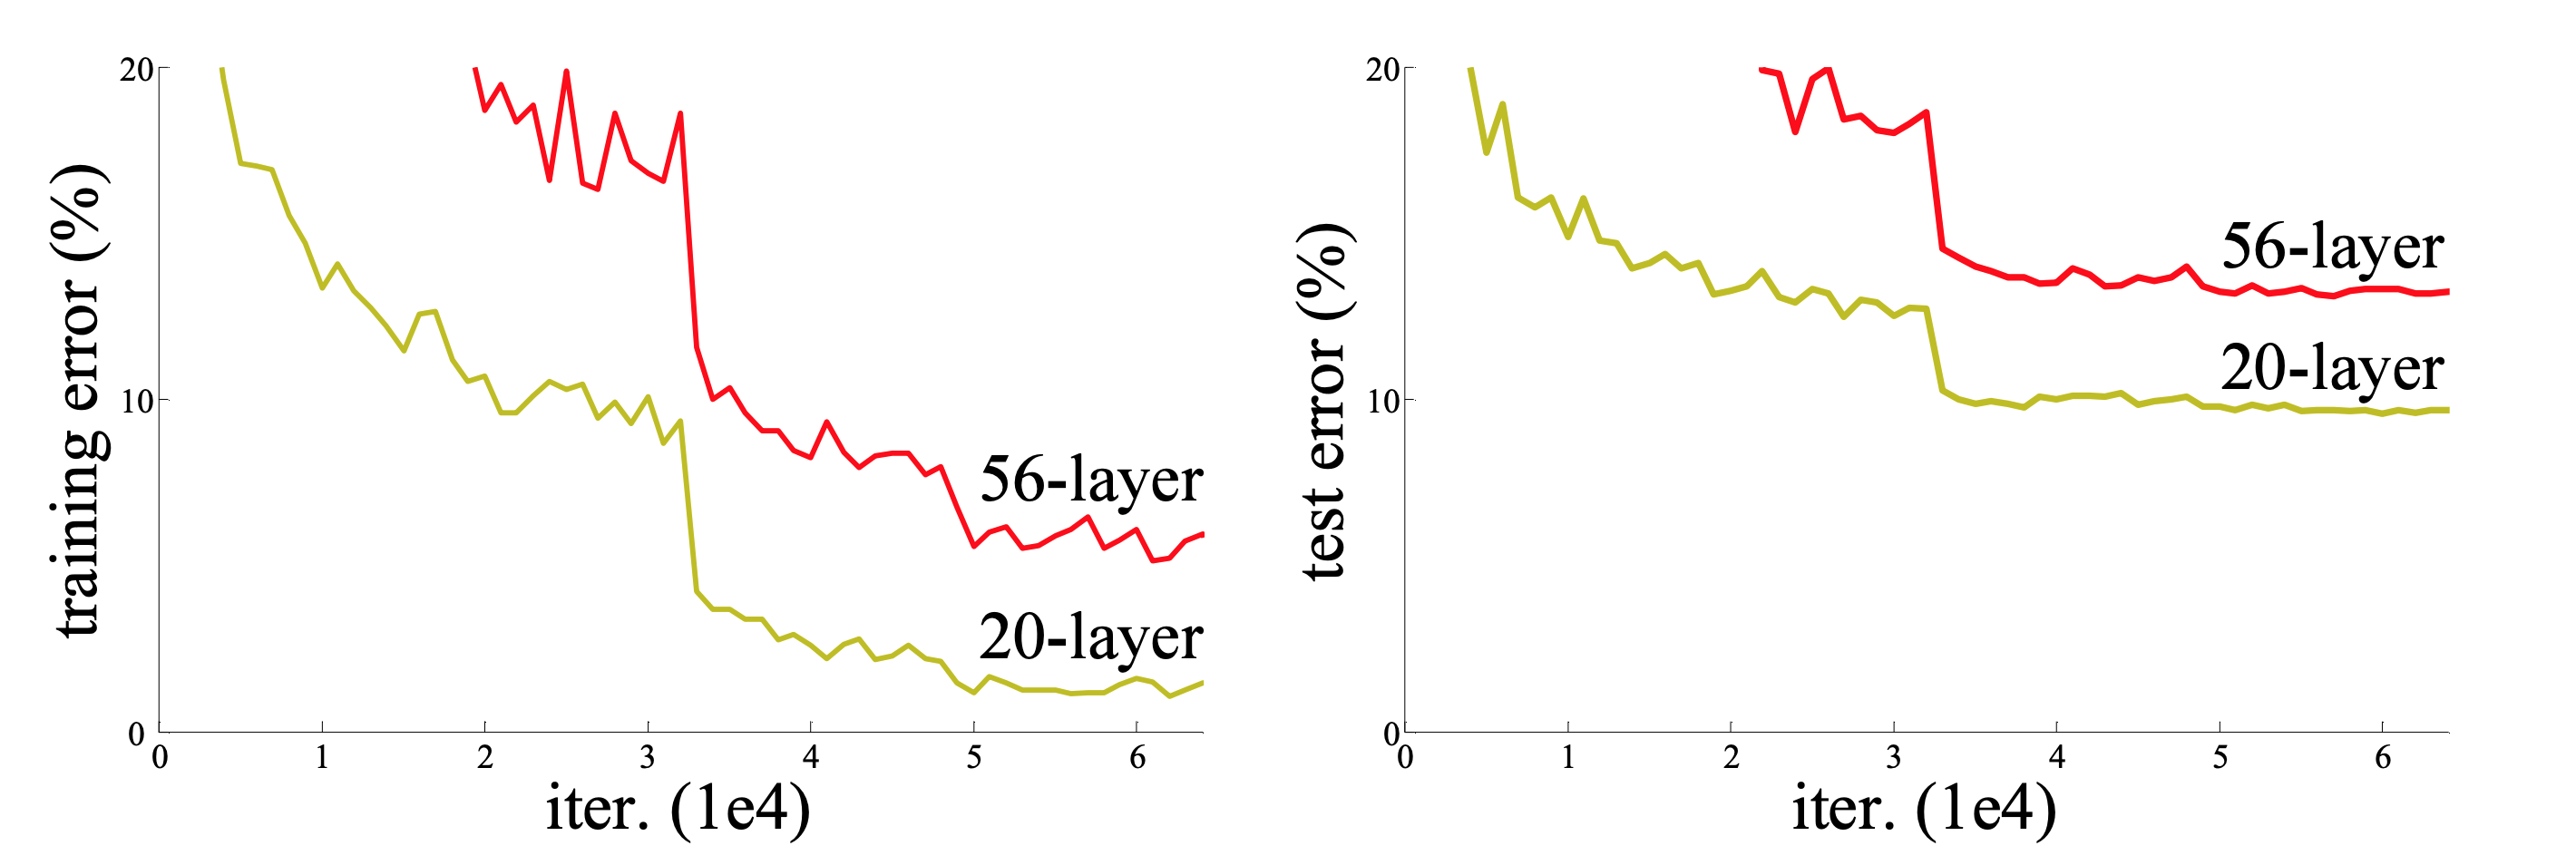
\includegraphics[scale=0.2]{resources/inception/deep-error.png}}
\caption{Błąd predykcji w stosunku do zastosowanej ilości iteracji treningowych przy uwzględnieniu ilości użytych warstw ukrytych dla standardowej architektury sieci neuronowej \cite{resnetpaper}.}
\label{fig:deep-error}
\end{figure}

Incepcja rozwiązuje ten problem rozbudowując się o dodatkowe operacje splotu w obrębie jednej warstwy-bloku (opisanego w podrozdziale \ref{subsection:inception-block}).
To wraz ze zastosowaniem operacji splotu o wymiarach filtra \(1 \times 1\) (rysunek \ref{fig:dlawik}), sprawiło, że można było zbudować sieć o jeszcze większej ilości warstw ukrytych, która jednocześnie zyskiwała na jakości predykcji.

\subsection{Blok sieci incepcja}
\label{subsection:inception-block}
Główną cechą sieci typu incepcja jest to, że jej architektura została rozbudowana o dodatkowe operacje splotu w obrębie jednej warstwy \ref{fig:inception-block}.
Mając do dyspozycji warstwę (lub \(N\) warstw) o wymiarach filtra \(W \times H\) stosujemy równocześnie splot o wymiarach filtra \(1 \times 1\), \(3 \times 3\), \(5 \times 5\) oraz warstwę MaxPool. 
Wynik tych operacji konkatenowany jest i zapisywany jako warstwa wyjściowa. Wykonywane operacje splotu mają tak dobrane krok i dopełnienia by wymiar \(W\) i \(H\) nie uległy zmianie. 
Taki dobór parametrów ma na celu łączenie jednego bloku sieci incepcja bezpośrednio w drugi podobnie jak ma to miejsce w przypadku warstw sieci VGG. 
Podobnie jak w przypadku VGG w celu modyfikacji dwóch pierwszych wymiarów warstwy stosowane są warstwy \textit{MaxPool} bezpośrednio między blokami incepcji.

\begin{figure}[ht]
\centerline{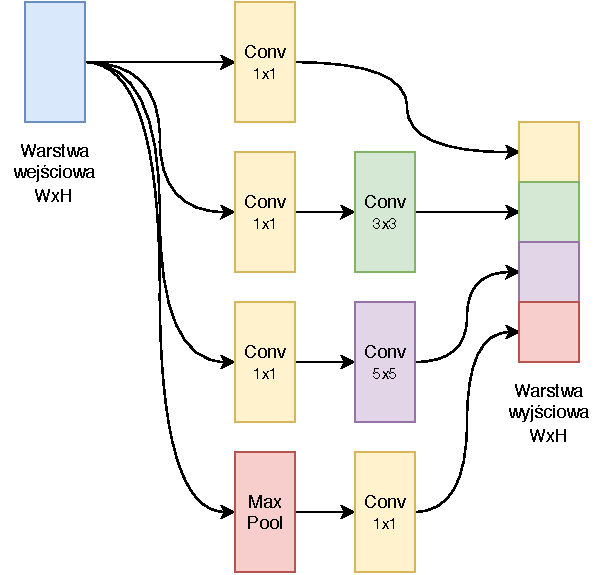
\includegraphics[scale=1]{resources/Inception_block.pdf}}
\caption{Schemat bloku z których składa się sieć incepcja.}
\label{fig:inception-block}
\end{figure}

Operacje splotu o wymiarach \(1 \times 1\) są stosowane przed \(3 \times 3\) i \(5 \times 5\) w celu redukcji liczby wartw filtrów co ma pozytywny wpływ na koszt obliczeniowy tej operacji \ref{fig:dlawik}.
Stosując \(F\) zestawów filtrów można dowolnie modyfikować trzeci wymiar uzyskanej warstwy. Dzięki temu, razem z MaxPool, splot \(1 \times 1\) pozwala na dowolną modyfikację wymiarów uzyskiwanych konwolucji.

\begin{figure}[ht]
\centerline{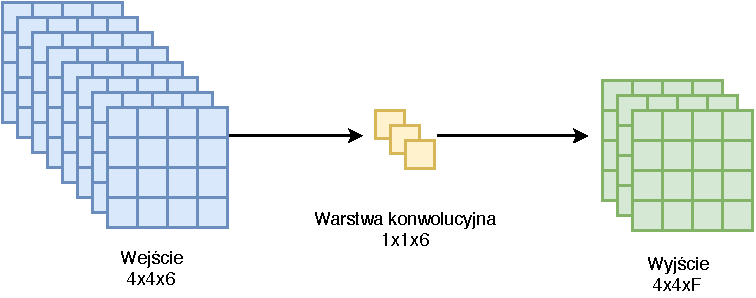
\includegraphics[scale=1]{resources/dlawik.pdf}}
\caption{Modyfikacja ilości warstw przy pomocy splotu \(1 \times 1\).}
\label{fig:dlawik}
\end{figure}

\subsection{Schemat sieci}

Zaprezentowany wariant sieci Incepcja, tak zwany GoogleLeNet \ref{fig:googleNet} to 22 warstwowa sieć konwolucyjna. Oprócz widocznych dla Incepcji bloków, GoogleLeNet posiada 3 osobne warstwy
wyjściowe typu softmax. Każde z tych wyjść używane jest w czasie treningu do obliczania funkcji kosztu (ich koszt dodawany jest do całkowitego kosztu z wagą 0,3).
Autorzy twierdzą, że taka operacja ma właściwości regularyzujące wagi oraz pomaga z problemem zanikającego gradientu występującego przy tak głębokich sieciach neuronowych.
Te dodatkowe wyjścia nie biorą udziału w procesie testowania ani podczas pracy z danymi produkcyjnymi.
Między warstwami konwolucyjnymi a gęstopołączonymi znajduje się pierwszy w tej pracy przykład użycia \textit{AveragePooling}. Autorzy podają, że takie stosowanie \textit{AveragePooling} zwiększył dokładność najlepszych predykcji o około 0.6\%.
Jako, że z racji wielkości nie sposób zamieścić wszystkich informacji na temat sieci w postaci znanych do tej pory z tej pracy diagramów, dokładne informacje na temat użytych warstw zawiera tabela na rysunku \ref{fig:googleNettable}.

\begin{figure}[ht]
\centerline{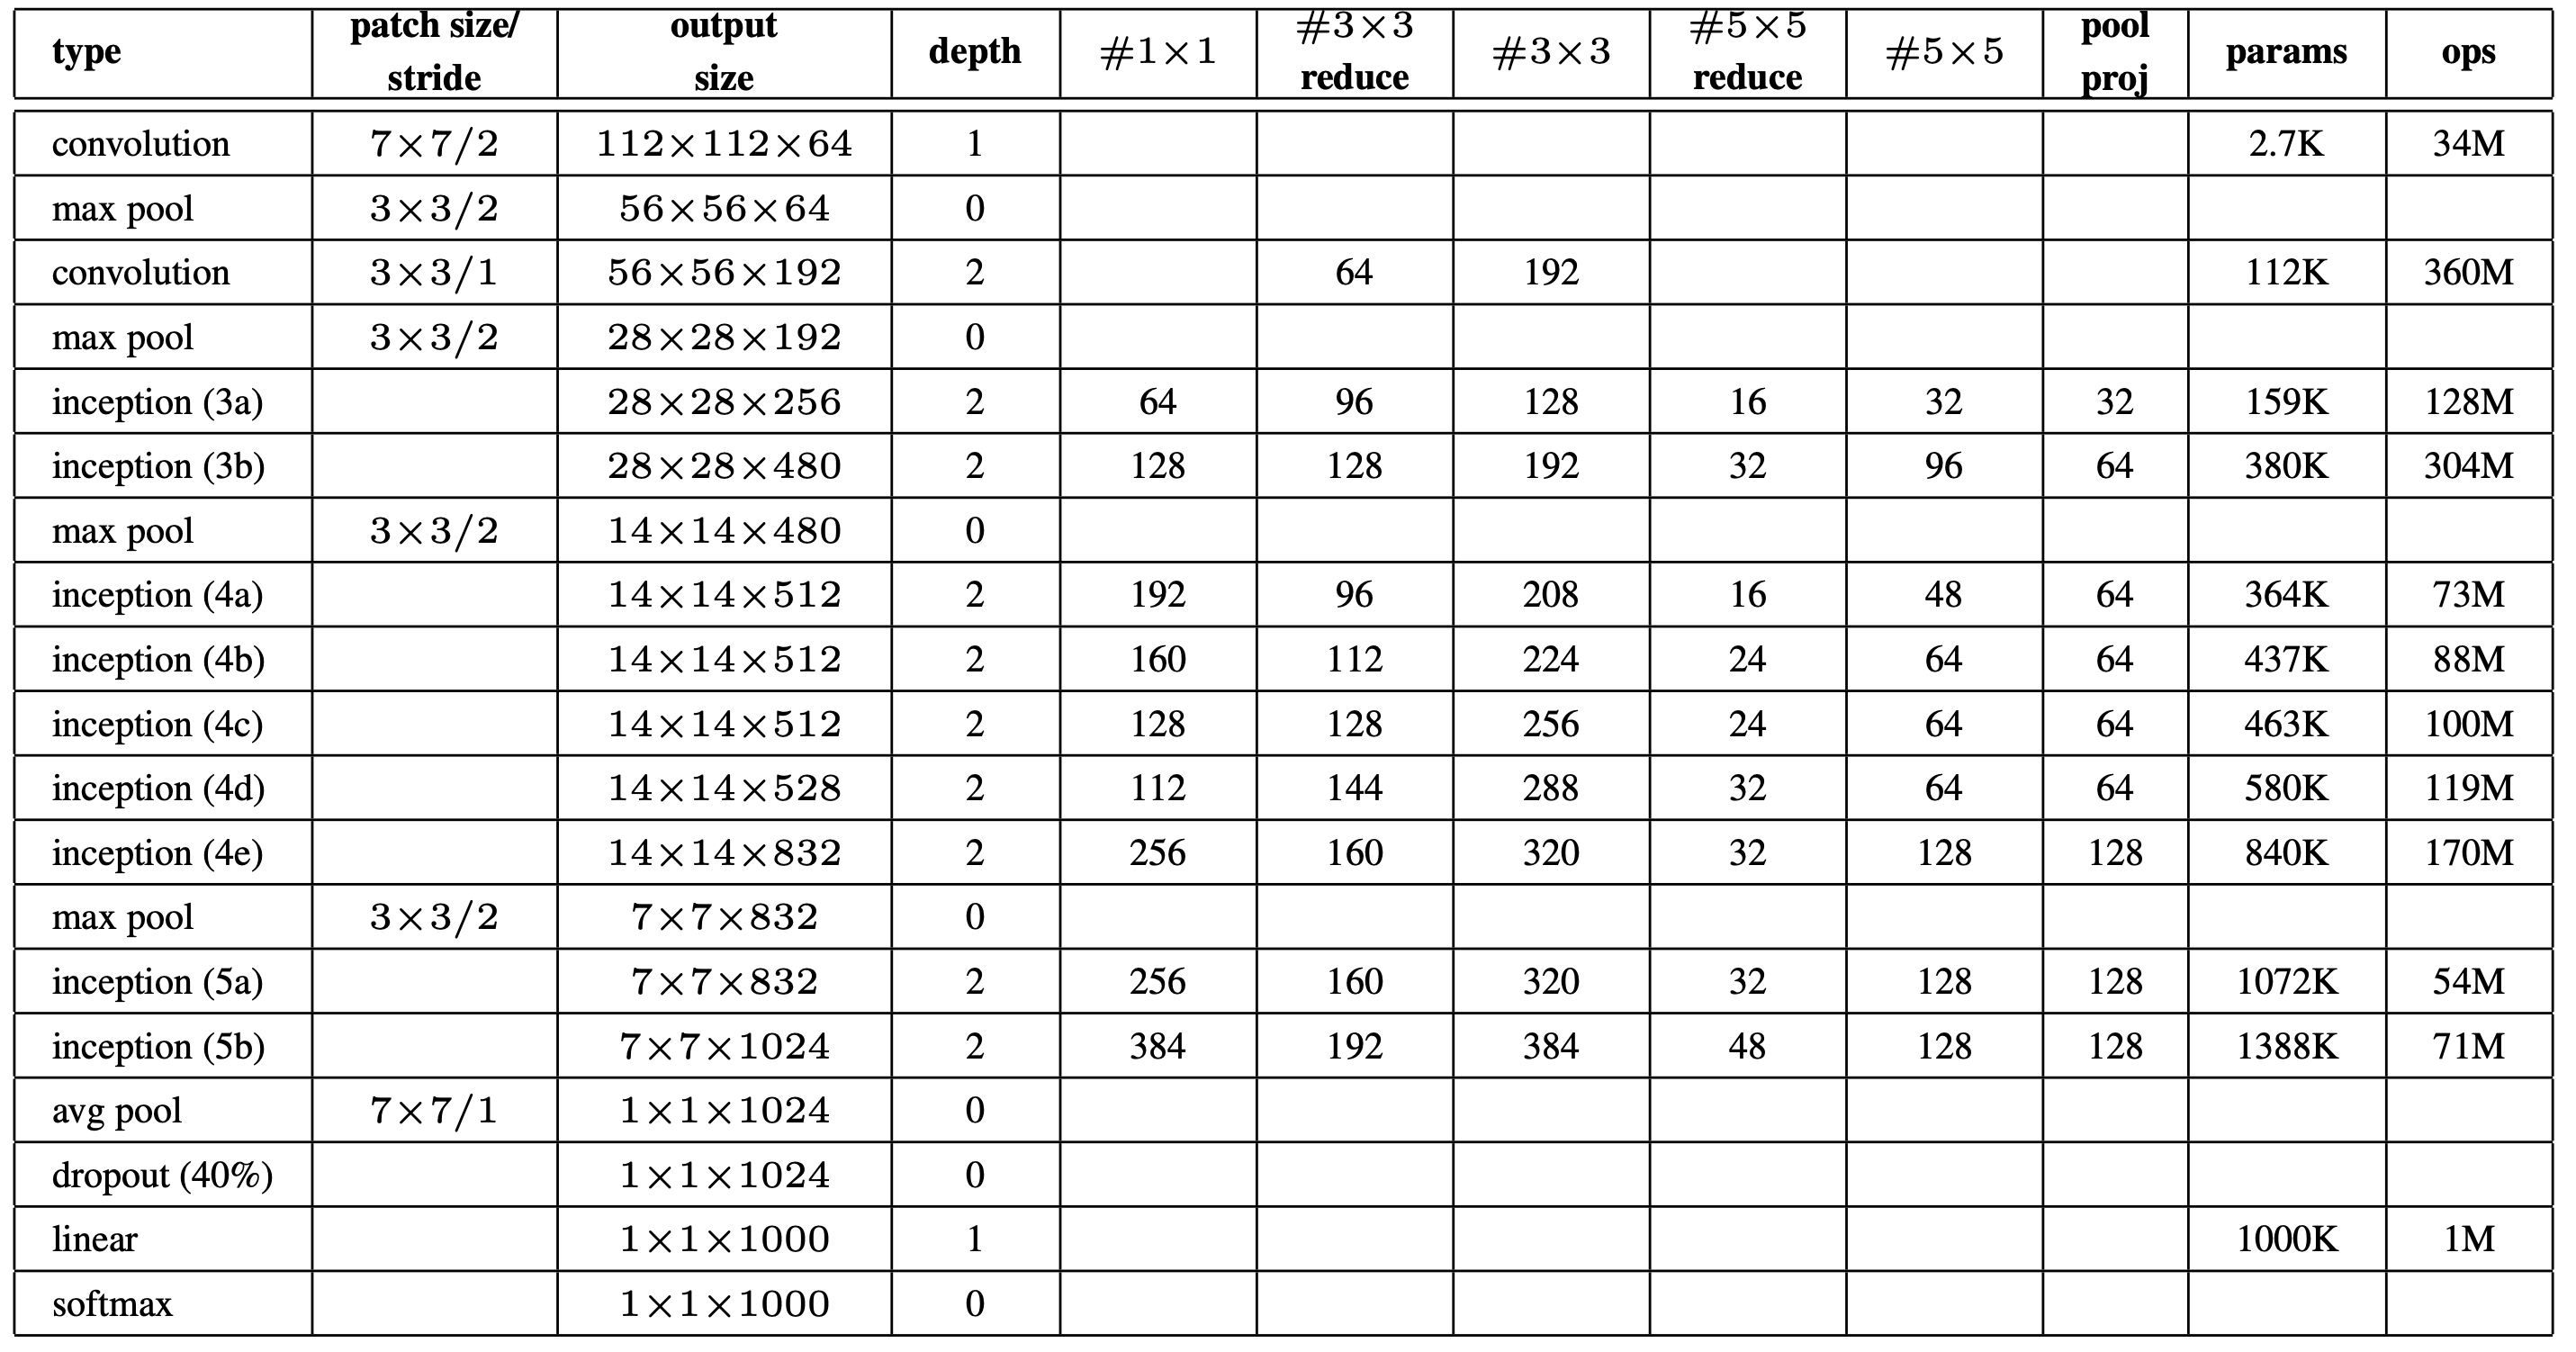
\includegraphics[scale=0.3]{resources/inception/googleNet-table.png}}
\caption{Szczegółowe dane na temat GoogleLeNet zaprezentowane w \textit{ang. Going deeper with convolutions} \cite{inceptionpaper}.} 
\label{fig:googleNettable}
\end{figure}

\begin{figure}[ht]
\centerline{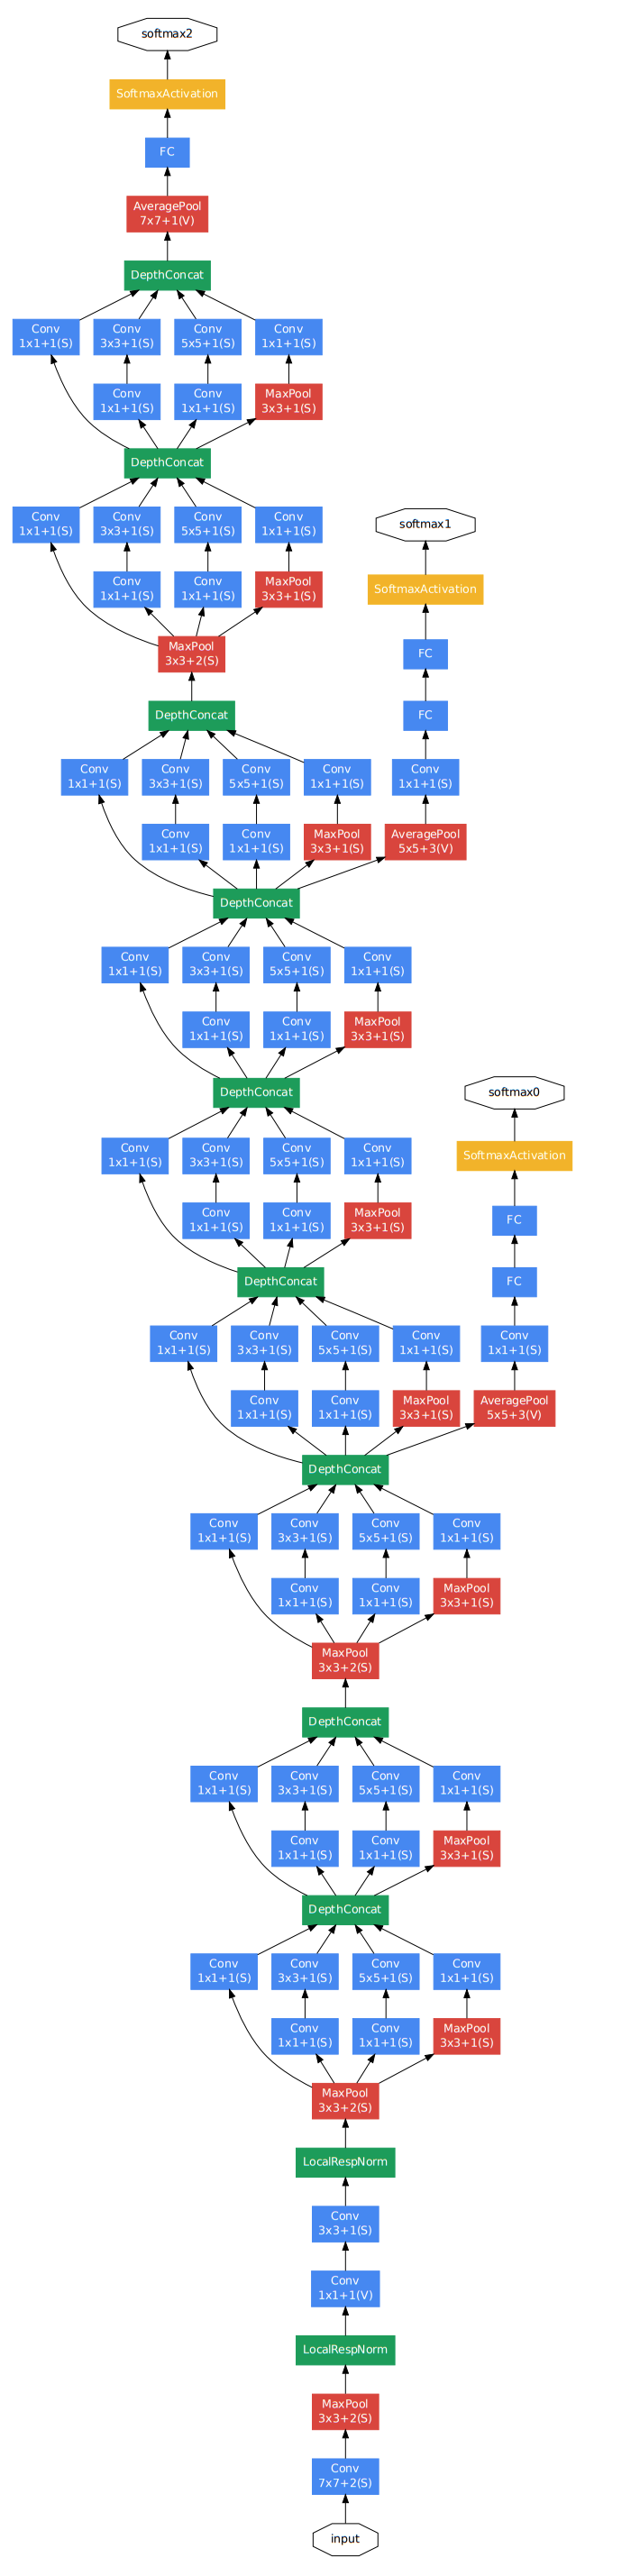
\includegraphics[scale=0.4]{resources/inception/googleNet.png}}
\caption{Schemat sieci GoogleLeNet zaprezentowany w \textit{ang. Going deeper with convolutions} \cite{inceptionpaper}.} 
\label{fig:googleNet}
\end{figure}

\section{\textit{DeepDream}}

\subsection{Opis i zasada działania}

\textit{DeepDream} to  program komputerowy stworzony przez Aleksandra Mordvintseva. Został opublikowany  w 2015 roku i opisany w formie posta na blogu \cite{deepdream}.

Co do zasady działania \textit{Deepdream} jest modyfikacją programu zaprezentowanego w podrozdziale \ref{vgg-mean-activation}. Podobnie jak w wyżej wymienionym programie, używając wcześniej wytrenowanej sieci neuronowej modyfikujemy obraz by zmaksymalizować aktywację neuronów danej sieci konwolucyjnej.

Poza oczywistą zamianą VGG na GoogleLeNet, \textit{DeepDream} stosuje znany już z podrozdziału
\ref{vgg-nst} sposób obliczania aktywacji kilku neuronów na raz przy użyciu paramteru stopnia 
użycia danej warstwy \(\lambda\). Obliczając aktywację dla kilku warstw na raz uzyskuje się bogatsze w treść efekty wizualne. Podobnie jak w przypadku wizualizacji uzyskanych na VGG, w celu uzyskania obrazu,
modyfikować wcześniej spreparowany, wylosowany obraz-szum. W swoim poście oryginalny autor posłużył się kolorowym obrazem (RGB). Najciekawsze efekty jednak uzyskano przy pomocy modyfikacji już istniejących zdjęć. Tak samo jak poprzednio, obraz jest wieloktronie skalowany podczas treningu, ale z racji swoich rozmiarów sieć GoogleLeNet jest w stanie uchwycić struktury obrazu nieuchwtyne dla VGG co umożliwia generowanie 
nieco psychodelicznych obrazów.

\subsection{Sposób uzyskiwania wizualizacji}
Choć \textit{DeepDream} może zostać zaimplementowany od podstaw przy pomocy \textit{Kerasa}, ja zdecydowałem się na  
opublikowaną przez Google, opartą na \textit{tensorflow}, bibliotekę \textit{lucid} \cite{lucidrepo}. Jej głównym zastosowaniem jest wizualizacja neuronów, ale pozwala też m.in na \textit{neural style transfer}, nawet na obiektch 3D.

\section{Nie oparty o VGG Neural Style Transfer na przykładzie sieci incepcja}
